\documentclass[letterpaper,11pt]{article}

\usepackage[utf8]{inputenc}
\usepackage[english]{babel}
\usepackage[empty]{fullpage}
\usepackage[usenames,dvipsnames]{color}
\usepackage{enumitem}
\usepackage{fancyhdr}
\usepackage{fontawesome}
\usepackage{geometry}
\usepackage{graphicx}
\usepackage[hidelinks]{hyperref}
\usepackage{textcomp}
\usepackage{titlesec}

\geometry{
	a4paper,
	left=20mm,
	right=20mm,
	top=15mm,
	bottom=15mm,
}

\pagestyle{fancy}
\fancyhf{}
\fancyfoot{}
\renewcommand{\headrulewidth}{0pt}
\renewcommand{\footrulewidth}{0pt}

\urlstyle{same}

\raggedbottom
\raggedright
\setlength{\tabcolsep}{0in}

\titlespacing{\section}{0pt}{15pt}{5pt}
\titleformat{\section}{
	\scshape\raggedright\large\bfseries
}{}{0em}{}[\color{black}\titlerule]

\newcommand{\resumeSubHeading}[1]{
	\item\textbf{#1}\vspace{-7pt}
}

\newcommand{\resumeTwoLineHeading}[4]{
	\item
	\begin{tabular*}{1.0\textwidth}[t]{l@{\extracolsep{\fill}}r}
		\textbf{#1} & \textbf{\small #2} \\
		\textit{\small #3} & \textit{\small #4} \\
	\end{tabular*}\vspace{-7pt}
}

\newcommand{\resumeProjectHeading}[3]{
	\item
	\begin{tabular*}{1.0\textwidth}{l@{\extracolsep{\fill}}r}
		\textbf{\small #1} $|$ \emph{\small #2} & \textbf{\small #3} \\
	\end{tabular*}\vspace{-7pt}
}

\newcommand{\resumeSubHeadingListStart}{\begin{itemize}[leftmargin=0.0in, label={}]}
\newcommand{\resumeSubHeadingListEnd}{\end{itemize}}
\newcommand{\resumeBlankListStart}{\begin{itemize}[leftmargin=0.15in, label={}]}
\newcommand{\resumeBlankListEnd}{\end{itemize}}
\newcommand{\resumeBulletListStart}{\begin{itemize}[leftmargin=0.3in]}
\newcommand{\resumeBulletListEnd}{\end{itemize}\vspace{-8pt}}
\newcommand{\resumeNumberedListStart}{\begin{enumerate}[leftmargin=0.35in]}
\newcommand{\resumeNumberedListEnd}{\end{enumerate}}	

\newcommand{\resumeItem}[1]{\item\small{{#1 \vspace{-2pt}}}}
\newcommand{\resumeSubItem}[1]{\resumeItem{#1}\vspace{-4pt}}

\renewcommand\labelitemi{$\vcenter{\hbox{\tiny$\bullet$}}$}
\renewcommand\labelitemii{$\vcenter{\hbox{\tiny$\bullet$}}$}


\begin{document}

\begin{tabular}{l c}
	\begin{minipage}{0.2\textwidth}
		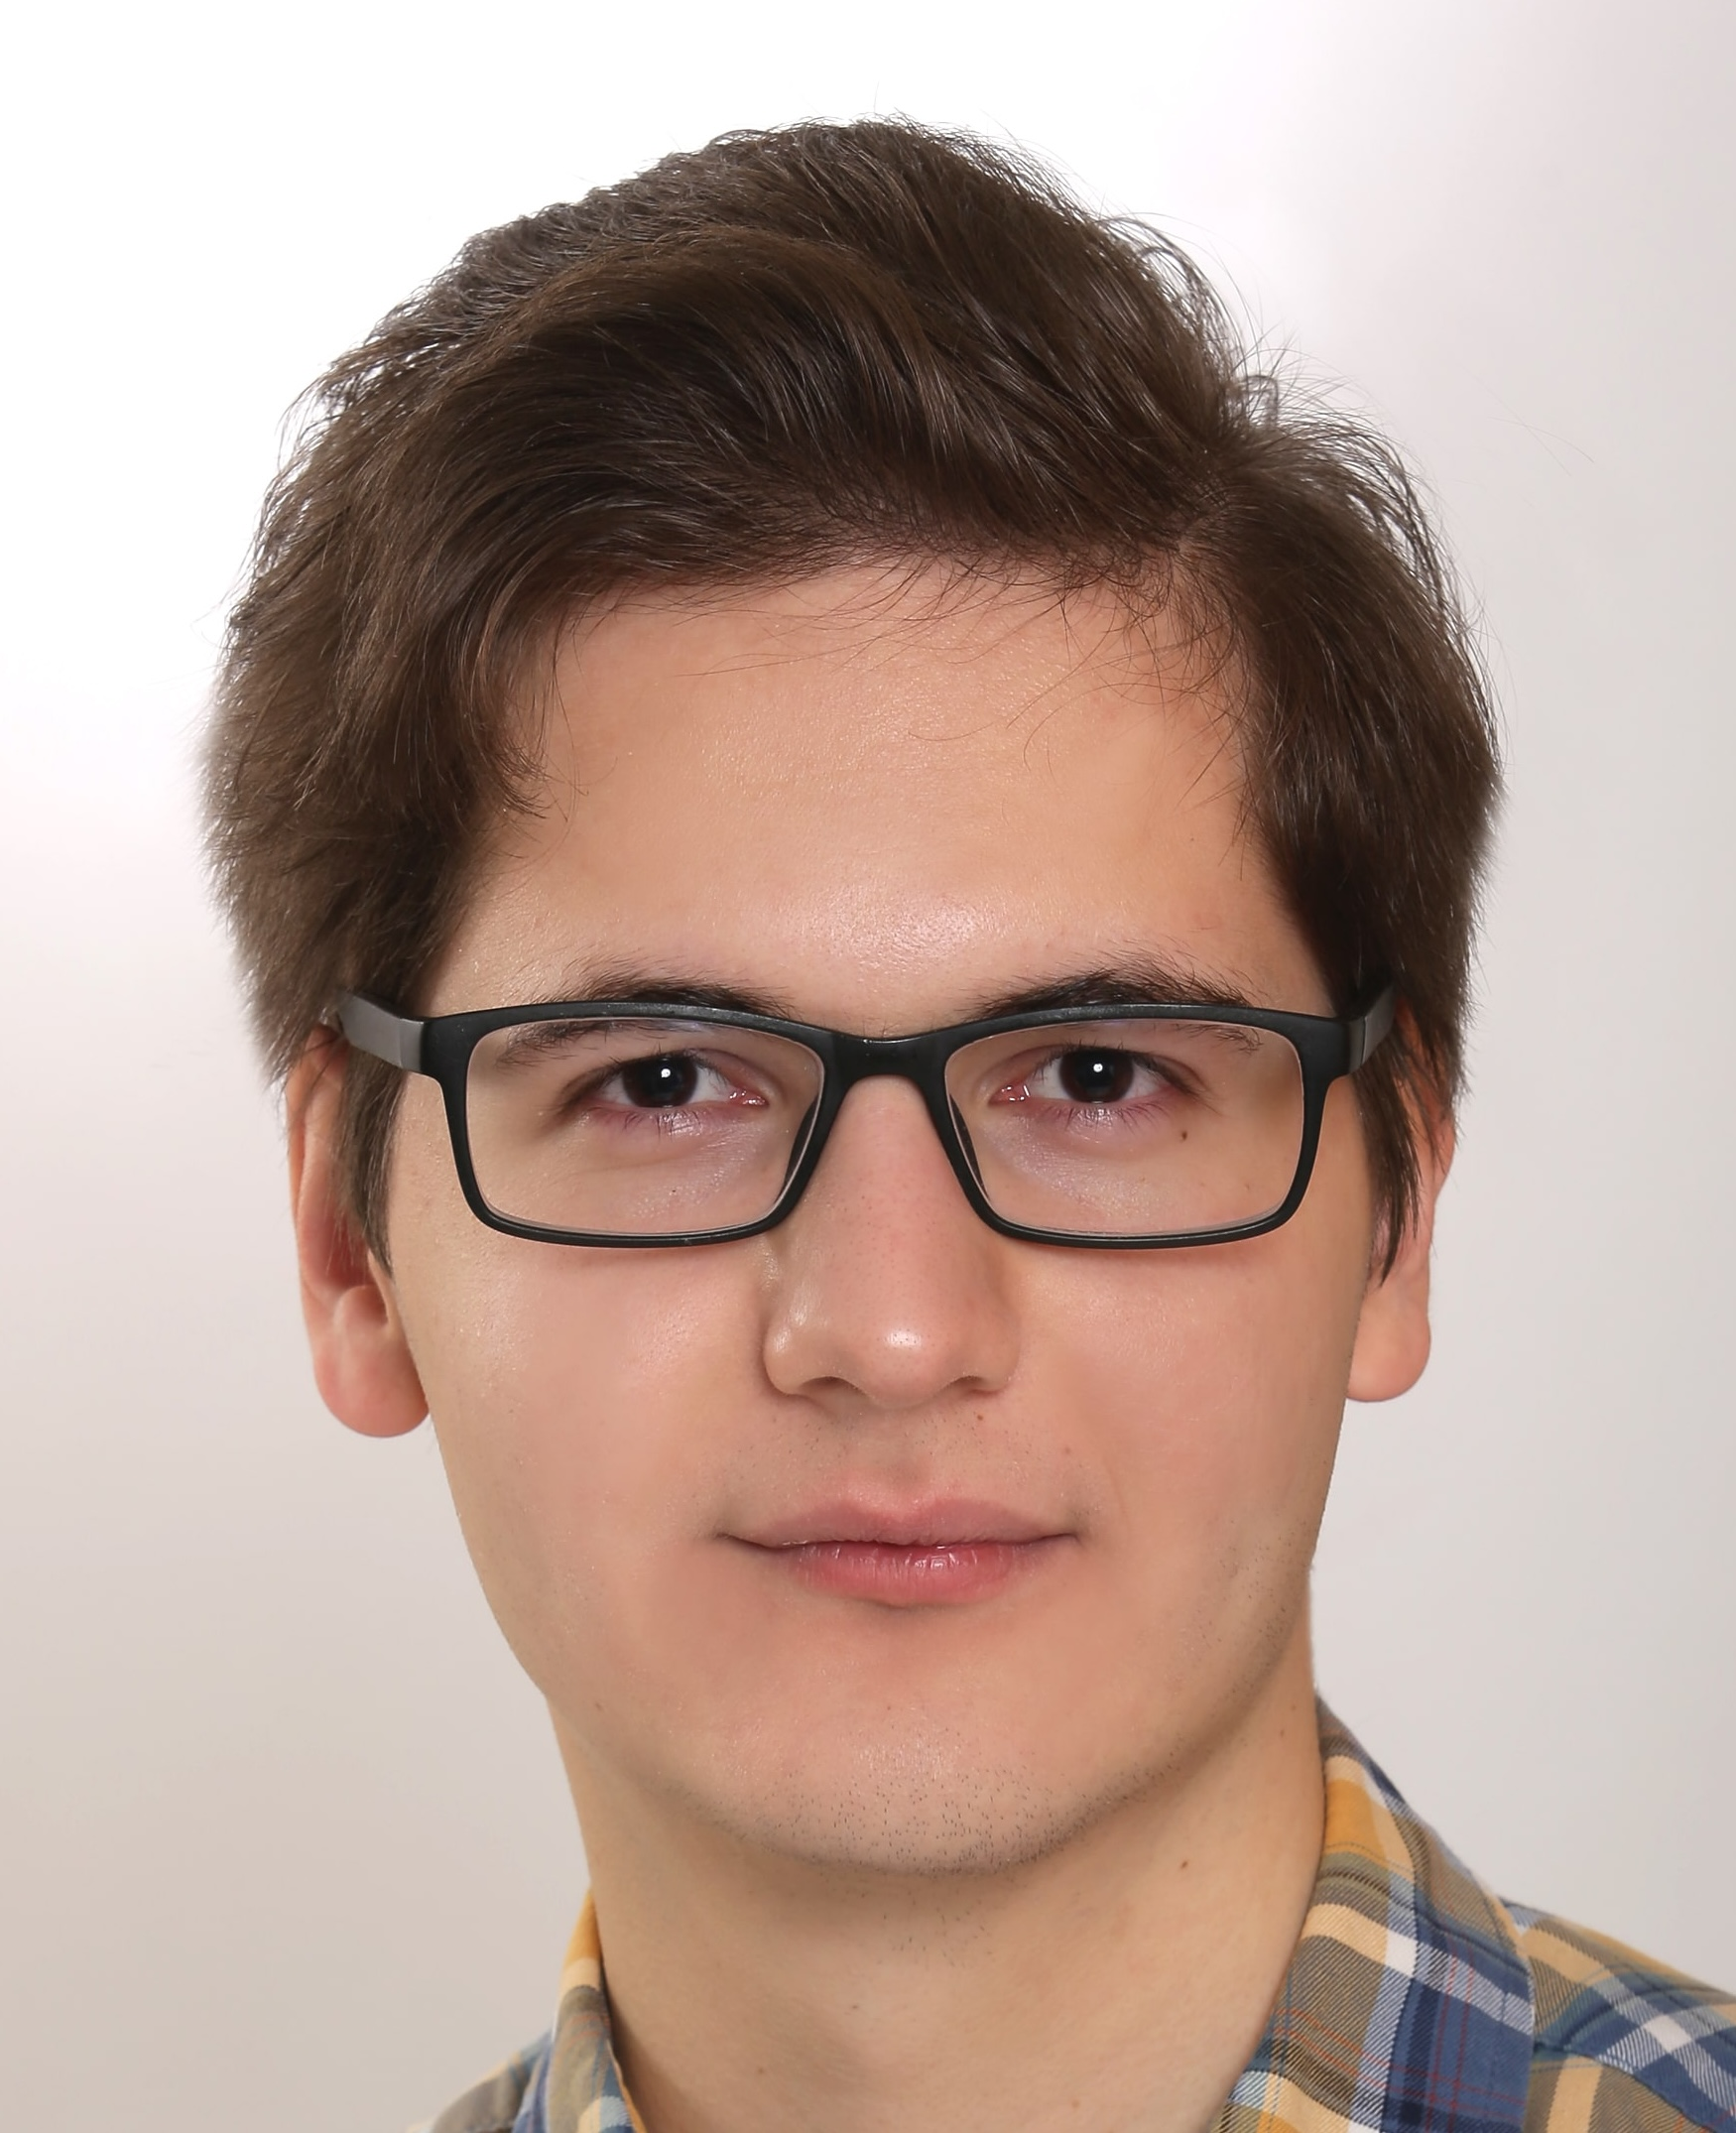
\includegraphics[width=\textwidth]{25.11.23-2.jpg}
	\end{minipage} &
	\begin{minipage}{0.65\textwidth}
	\begin{center}
		\vspace{15pt}
		{\Huge \scshape Fedor Kuyanov} \\ 
		\vspace{15pt}
		\small \raisebox{-0.1\height}\faHome\ Moscow, Russia ~ 
		\small \raisebox{-0.1\height}\faPhone\ +7 (926) 780-75-40 ~ \\
		\vspace{5pt}
		\href{mailto:feodor.kuyanov@gmail.com}{\raisebox{-0.2\height}\faEnvelope\  \underline{feodor.kuyanov@gmail.com}} ~ 
		\href{https://github.com/kuyanov}{\raisebox{-0.2\height}\faGithub\ \underline{github.com/kuyanov}}
	\end{center}
	\end{minipage}
\end{tabular}


\section{Education}

\resumeSubHeadingListStart

\resumeTwoLineHeading
{HSE University}{September 2020 -- July 2024}
{BSc majoring in Theoretical Computer Science, GPA 9.8/10, rank 1/260}{Moscow, Russia}

\resumeSubHeading{Summer schools}
\resumeBulletListStart
\resumeItem{\href{https://mccme.ru/dubna/eng/}{\underline{Contemporary Mathematics}} (Dubna, Russia, 2019)}
\resumeItem{\href{https://in.harbour.space/tech-scouts/}{\underline{Harbour.Space Tech Scouts}} (Barcelona, Spain, 2019)}
\resumeItem{\href{https://www.turgor.ru/en/lktg/index.php}{\underline{Summer Conference of the Mathematical Tournament of Towns}} (Serbia, 2019)}
\resumeItem{\href{http://lksh.ru}{\underline{Summer Computer School}} (Russia, 2014 -- 2017, levels C', B', B, A)}
\resumeBulletListEnd

\resumeSubHeadingListEnd


\section{Work experience}

\resumeSubHeadingListStart

\resumeTwoLineHeading
{HSE, Laboratory of Theoretical Computer Science}{September 2021 -- present}
{Research assistant}{Moscow, Russia}
\resumeBulletListStart
\resumeItem{Research in mathematical physics and number theory: quantum walks.}
\resumeItem{Research in linear algebra and complexity theory: minimizing the number of operations for matrix multiplication.}
\resumeBulletListEnd

\resumeTwoLineHeading
{EPFL, Laboratory of Theoretical Computer Science}{July 2023 -- September 2023}
{Research assistant}{Lausanne, Switzerland}
\resumeBulletListStart
\resumeItem{Research in randomized sublinear algorithms on graphs such as bipartiteness testing.}
\resumeBulletListEnd

\resumeTwoLineHeading
{Moscow State School №57}{September 2022 -- December 2022}
{Teaching assistant}{Moscow, Russia}
\resumeBulletListStart
\resumeItem{Assisted calculus and programming classes in Moscow State School №57, one of the top math schools in Russia.}
\resumeBulletListEnd

\resumeTwoLineHeading
{Huawei}{June 2022 -- December 2022}
{Software Engineer}{Moscow, Russia}
\resumeBulletListStart
\resumeItem{Member of the graph computing team focused on fluid and gas processes simulation on  lattices.}
\resumeItem{Implemented distributed versions of the Conjugate gradient method and Lanczos algorithm.}
\resumeBulletListEnd

\resumeTwoLineHeading
{Yandex}{May 2021 -- August 2021}
{Software Engineer Intern}{Moscow, Russia}
\resumeBulletListStart
\resumeItem{Enhanced scenario classification of the voice assistant Alice by adapting the learning process for different devices.}
\resumeBulletListEnd

\resumeTwoLineHeading
{Summer informatics workshop}{June 2020}
{Teaching assistant}{Moscow, Russia}
\resumeBulletListStart
\resumeItem{Prepared Russian national team candidates to IOI by creating practice contests and tutorials.}
\resumeBulletListEnd

\resumeSubHeadingListEnd


\section{Publications}

\resumeNumberedListStart
\resumeSubItem{\href{https://www.worldscientific.com/doi/10.1142/S0129055X23500228}{Feynman checkers: number-theoretic properties} (joint paper with A. Slizkov). \textit{Reviews in Mathematical Physics}, 35:09 (2023) 2350022, \href{https://arxiv.org/abs/2210.07306}{arXiv:2210.07306}}
\resumeNumberedListEnd


\section{Conference talks}

\resumeBulletListStart
\resumeSubItem{\href{https://confhub.ru/eng/event/7500/}{\underline{29th International Scientific Conference ``Lomonosov''}} (Moscow, Russia, 2022)}
\resumeSubItem{\href{https://cms-math.net.technion.ac.il/files/2023/03/workshop-4.pdf}{\underline{Diophantine Analysis, Dynamics, and related topics}} (Haifa, Israel, 2023)}
\resumeBulletListEnd


\section{Projects}

\resumeSubHeadingListStart

\resumeProjectHeading
{\href{https://github.com/Qock-Foundation/matrix-multiplication}{\underline{MatrixMultiplication}}}{Python, PyTorch}{October 2023}
\resumeBulletListStart
\resumeItem{Python scripts generating optimal matrix multiplication algorithms for small sizes (up to 3).}
\resumeItem{Uses modern optimization techniques from machine learning and performs greedy rounding to get rational coefficients.}
\resumeBulletListEnd

\resumeProjectHeading
{\href{https://github.com/kuyanov/wordle}{\underline{Wordle}}}{C++, JavaScript}{August 2022}
\resumeBulletListStart
\resumeItem{The goal of this game is to guess a 5-letter word in 6 tries based on the information about each letter.}
\resumeItem{Implemented a strategy (using B\&B algorithm and information theory) that achieves the world record of \href{https://auction-upload-files.s3.amazonaws.com/Wordle_Paper_Final.pdf}{\underline{3.42 tries}}.}
\resumeBulletListEnd

\resumeProjectHeading
{\href{https://github.com/m20-sch57/fejudge}{\underline{Fejudge}}}{Python, Linux kernel}{September 2021}
\resumeBulletListStart
\resumeItem{This is a management system for programming contests with a convenient web interface.}
\resumeItem{Uses various Linux kernel features (such as cgroups) and supports simultaneous evaluation on different machines.}
\resumeBulletListEnd

\resumeProjectHeading
{\href{https://github.com/m20-sch57/thetruehat}{\underline{TheTrueHat}}}{JavaScript, Vue}{August 2021}
\resumeBulletListStart
\resumeItem{This project allows playing the Hat (Alias) game from the browser.}
\resumeBulletListEnd

\resumeProjectHeading
{\href{https://github.com/JaggedLine/kotline}{\underline{Kotline}}}{Kotlin, React, JavaScript}{January 2021}
\resumeBulletListStart
\resumeItem{Geometric puzzle where one must build the longest non-self-intersecting polygonal chain.}
\resumeBulletListEnd

\resumeSubHeadingListEnd


\section{Skills \& interests}

\resumeBlankListStart
\resumeSubItem{\textbf{Programming languages: }{C/C++, Python, Kotlin, HTML/CSS, JavaScript, Bash, SQL}}
\resumeSubItem{\textbf{Libraries \& frameworks: }{QT, NumPy, matplotlib, pandas, PyTorch, Flask, React, Vue}}
\resumeSubItem{\textbf{Tools: }{CI/CD, git, docker, gdb, cmake}}
\resumeSubItem{\textbf{Interested in: }{quantum computing, algorithms and complexity theory, linear algebra, discrete math}}
\resumeBlankListEnd


\section{Scholarships \& grants}

\resumeBulletListStart
\resumeSubItem{\href{https://cs.hse.ru/en/stipend}{\underline{Ilya Segalovich Scholarship}}, twice (2022, 2023)}
\resumeSubItem{\href{https://www.tinkoff.ru/about/news/06042022-tinkoff-launches-scholarship-programme-for-russias-young-talent-eng/}{\underline{Tinkoff Scholarship}} (2022)}
\resumeSubItem{Research and educational group ``Combinatorial and numerical problems on lattices'' (HSE, 2023)}
\resumeSubItem{Project group ``Lattice models'' (HSE, 2020 -- 2022)}
\resumeBulletListEnd


\section{Competitions}

\resumeBulletListStart
\resumeSubItem{Three times gold medal at \href{https://imc-math.org.uk}{\underline{IMC}} (2021 -- 2023)}
\resumeSubItem{Silver medal at \href{https://neerc.ifmo.ru/archive/2020.html}{\underline{Semifinal ICPC 2020, NERC}}}
\resumeSubItem{Winner of several inter-university math competitions: \href{https://iuhd.edu.tm/competition/44}{\underline{NCUMC}}, \href{https://iuhd.edu.tm/competition/45}{\underline{OMOUS}}, \href{http://www.rkarasev.ru/note/66}{\underline{MIPT}}, \href{https://cs.hse.ru/en/announcements/504365867.html}{\underline{OSAM Comp'21}}}
\resumeSubItem{Prize-winner of the All-Russian Olympiad in Mathematics (2018, 2019, 2020)}
\resumeSubItem{Winner of the All-Russian Olympiad in Informatics (2018), prize-winner in 2017, 2019, 2020}
\resumeSubItem{Six times winner of the \href{https://www.turgor.ru/en/}{\underline{International Mathematical Tournament of Towns}} (2014 - 2019)}
\resumeSubItem{Grand prix and first prize at the international piano competition CMF 2015 (\href{https://www.youtube.com/watch?v=mFGwCgjjaP8}{\underline{YouTube}})}
\resumeBulletListEnd


\section{Hobbies}

\resumeBulletListStart
\resumeSubItem{Railway modeling, Lego}
\resumeSubItem{Chess, speed-cubing (3x3, 36 secs), ping-pong}
\resumeSubItem{Classical piano -- finished 8-year Gnesin music school and performed with an orchestra, \href{https://www.youtube.com/watch?v=KPUQTMAy0bQ&list=PL3n6QsMnv3lZyL8XD4WcQh4mhJ-REqBKN}{\underline{YouTube}}}
\resumeBulletListEnd


\section{Languages}

\resumeBulletListStart
\resumeSubItem{English: C1 (IELTS 7.5)}
\resumeSubItem{Russian: Native speaker}
\resumeBulletListEnd


\end{document}
